\date{}
\title{}
\date{}
\begin{document}
\begin{frame}
    \titlepage
\end{frame}

\input{../common/listingsLib}

\begin{frame}
    \frametitle{last time}
    \begin{itemize}
        \item barriers
            \begin{itemize}
                \item Init(ThreadCount); Wait() [for all other threads]
                \item reusable
            \end{itemize}
        \item monitors (start)
            \begin{itemize}
            \item lock(Lock);
            \item while (need to wait b/c of shared data) Wait(CV, Lock); 
            \item do something with shared data
            \item if (someone can stop waiting) Broadcast/Signal(CV)
            \item unlock(Lock)
            \end{itemize}
    \end{itemize}
\end{frame}

\subsection{exercise: wait for both finished}
\usetikzlibrary{arrows.meta}
\begin{frame}[fragile,label=bothFinishedEx]{wait for both finished}
\begin{lstlisting}[
    language=C++,style=size105,
    morekeywords={pthread_mutex_t,pthread_cond_t},
    moredelim={**[is][\btHL<2|handout:2>]{@2}{2@}}, 
    moredelim={**[is][\btHL<3|handout:3>]{@3}{3@}}, 
    moredelim={**[is][\btHL<4|handout:4>]{@4}{4@}}, 
    moredelim={**[is][\btHL<5|handout:5>]{@5}{5@}}, 
    escapeinside=QQ,
]
// MISSING: init calls, etc.
pthread_mutex_t lock;
bool finished[2];
pthread_cond_t both_finished_cv;

void WaitForBothFinished() {
  pthread_mutex_lock(&lock);Q\tikzmark{lock for wait}Q
  while (@2_____________________________2@) {Q\tikzmark{finished loop}Q
    pthread_cond_wait(&both_finished_cv, &lock);Q\tikzmark{wait}Q
  }
  pthread_mutex_unlock(&lock);
}

void Finish(int index) {
  pthread_mutex_lock(&lock);Q\tikzmark{lock for finish}Q
  finished[index] = true;
  @3_____________________________________3@
  pthread_mutex_unlock(&lock);
}
\end{lstlisting}
\begin{tikzpicture}[overlay,remember picture]
\tikzset{
    >=Latex,
    explain box/.style={draw=red,text=black,very thick,align=left,font=\small},
    point line/.style={very thick,red},
}
\begin{visibleenv}<2>
    \node[explain box,anchor=north east] (acquire text) at ([yshift=-1cm,xshift=-.25cm]current page.north east) {
        A. \lstinline*finished[0] && finished[1]* \\
        B. \lstinline*finished[0] || finished[1]* \\
        C. \lstinline*!finished[0] || !finished[1]* \\
        D. \lstinline*finished[0] != finished[1]* \\
        E. something else
    };
\end{visibleenv}
\begin{visibleenv}<3>
    \node[explain box,anchor=north east,font=\fontsize{9}{10}\selectfont,fill=white] (acquire text) at ([yshift=-2cm,xshift=-.25cm]current page.north east) {
        A. \lstinline*pthread_cond_signal(&both_finished_cv)* \\
        B. \lstinline*pthread_cond_broadcast(&both_finished_cv)* \\
        C. \lstinline*if (finished[1-index])* \\
        \hspace{1.5cm} \lstinline*pthread_cond_signal(&both_finished_cv);* \\
        D. \lstinline*if (finished[1-index])* \\
        \hspace{1.5cm} \lstinline*pthread_cond_broadcast(&both_finished_cv);* \\
        E. something else
    };
\end{visibleenv}
\end{tikzpicture}
\end{frame}


\subsection{exercise: barrier}
\begin{frame}[fragile,label=monitorExercise2]{monitor exercise: barrier}
\begin{itemize}
\item suppose we want to implement a one-use barrier; fill in blanks:
\end{itemize}
\begin{lstlisting}[style=smaller]
struct BarrierInfo {
    pthread_mutex_t lock;
    int total_threads;  // initially total # of threads
    int number_reached; // initially 0
    ___________________
};

void BarrierWait(BarrierInfo *b) {
    pthread_mutex_lock(&b->lock);
    ++b->number_reached;
    if (b->number_reached == b->total_threads) {
        _____________________
    } else {
        _____________________
    }
    pthread_mutex_unlock(&b->lock);
}
\end{lstlisting}
\end{frame}


\section{reader-writer problem}
\begin{frame}{reader/writer problem}
    \begin{itemize}
    \item some shared data 
    \item only one thread modifying (read+write) at a time
    \item read-only access \myemph{from multiple threads} is safe
    \vspace{.5cm}
    \item<2-> could use lock --- but doesn't allow multiple readers
    \end{itemize}
\end{frame}

\section{rwlocks}
\begin{frame}{reader/writer locks}
\begin{itemize}
\item abstraction: lock that distinguishes readers/writers
\item operations:
    \begin{itemize}
    \item read lock: wait until no writers
    \item read unlock: stop being registered as reader
    \item write lock: wait until \myemph<2>{no readers and no writers}
    \item write unlock: stop being registered as writer
    \end{itemize}
\end{itemize}
\end{frame}

\begin{frame}[fragile,label=pthreadrwlock]{pthread rwlocks}
\begin{lstlisting}[language=C++,style=smaller]
pthread_rwlock_t rwlock;
pthread_rwlock_init(&rwlock, NULL /* attributes */);
...
    pthread_rwlock_rdlock(&rwlock);
    ...  /* read shared data */
    pthread_rwlock_unlock(&rwlock);

    pthread_rwlock_wrlock(&rwlock);
    ...  /* read+write shared data */
    pthread_rwlock_unlock(&rwlock);

...
pthread_rwlock_destroy(&rwlock);
\end{lstlisting}
\end{frame}



\begin{frame}[fragile]{transactions}
    \begin{itemize}
    \item transaction: set of operations that occurs atomically
    \item idea: something higher-level handles locking, etc.:
   \end{itemize}
\begin{Verbatim}
BeginTransaction();
int FromOldBalance = GetBalance(FromAccount);
int ToOldBalance = GetBalance(ToAccount);
SetBalance(FromAccount, FromOldBalance - 100);
SetBalance(ToAccount, FromOldBalance + 100);
EndTransaction();
\end{Verbatim}
    \begin{itemize}
    \item idea: library/database/etc. makes ``transaction'' happens all at once
    \end{itemize}
\end{frame}

\begin{frame}{consistency / durability}
    \begin{itemize}
    \item ``happens all at once'' = could mean:
    \vspace{.5cm}
    \item locking to make sure no other operations interfere (consistency)
    \item making sure on crash, no partial transaction seen (durability)
    \vspace{.5cm}
    \item \small (some systems provide both, some provide only one)
    \end{itemize}
\end{frame}


\begin{frame}
\frametitle{transaction implementation ideas}
\begin{itemize}
\item simple idea: do one transaction at a time
\item more efficient(?) idea: 
    \begin{itemize}
    \item get list of operations 
    \item lock everything operations use (in consistent order to prevent deadlock)
    \item do operations on list
    \item unlock everything
    \end{itemize}
\item (also other strategies with different flexibility/efficiency)
\end{itemize}
\end{frame}

\begin{frame}
\frametitle{networking}
\end{frame}




\section{mailbox model}

\usetikzlibrary{arrows.meta,shapes.symbols,shapes.multipart}

\begin{frame}{mailbox model}
    \begin{itemize}
    \item \textit{mailbox} abstraction: send/receive messages
    \end{itemize}
    \begin{tikzpicture}
    \tikzset{
        >=Latex,
        comp box/.style={draw, thick, align=center, minimum width=1.5cm,minimum height=3cm},
        explain box/.style={draw=red,very thick, align=left},
        msg/.style={font=\small},
        cmd/.style={font=\small},
    }
        \node[comp box] (machine A) at (-6.5, 0) {machine \\ A};
        \node[draw,cloud,line width=1pt,minimum width=4cm,minimum height=1cm,aspect=3,
                alt=<2>{red,thick}] (network) at (0,0) {the network};
        \node[comp box] (machine B) at (6.5, 0) {machine \\ B};
        \draw[very thick,->] (machine A) -- (network) 
            node[midway,above,msg] {B: ``Hello''}
            node[pos=0.0,below right,cmd] {Send(B, ``Hello'')};
        \draw[very thick,<-] (machine B) -- (network) 
            node[midway,above,msg] {B: ``Hello''}
            node[pos=0.0,below left,cmd] {Recv() = ``Hello''};
        % FIXME: hilite network: knows how to get message to particular place
            % note/show buffering at A/B
        \begin{visibleenv}<2>
            \node[explain box,anchor=north] at ([yshift=-.25cm]network.south) {
                network knows how to get message to B
            };
        \end{visibleenv}
        \begin{visibleenv}<3->
            \node[anchor=south,draw,rectangle,rectangle split,rectangle split parts=5,rectangle split horizontal, inner sep=0.25mm] at ([yshift=.1cm]machine A.south) {
                ~~~
            };
        \end{visibleenv}
        \begin{visibleenv}<3>
            \node[explain box,anchor=north] at ([yshift=-.25cm]network.south) {
                queue of messages \\
                from sending program \\
                waiting to be sent
            };
        \end{visibleenv}
        \begin{visibleenv}<4->
            \node[anchor=south,draw,rectangle,rectangle split,rectangle split parts=5,rectangle split horizontal,inner sep=0.25mm] at ([yshift=.1cm]machine B.south) {
                ~~~
            };
        \end{visibleenv}
        \begin{visibleenv}<4>
            \node[explain box,anchor=north] at ([yshift=-.25cm]network.south) {
                queue of messages \\
                not yet received by \\
                receiving program
            };
        \end{visibleenv}
    \end{tikzpicture}
\end{frame}

\begin{frame}{connections over mailboxes}
    \begin{itemize}
    \item real Internet: mailbox-style communication
        \begin{itemize}
        \item send packets to particular mailboxes
        \item no gaurentee on order, when received
        \end{itemize}
    \item sockets implemented on top of this
    \end{itemize}
\end{frame}


 % FIXME: wrong place?

\section{review: connection abstraction}

\input{../network/connection-model}

\section{recall: sockets}

\begin{frame}{recall: sockets}
    \begin{itemize}
    \item open connection then \ldots \\
    \item read+write just like a terminal file
    \vspace{.5cm}
    \item doesn't look like individual messages
    \item ``connection abstraction''
    \end{itemize}
\end{frame}

\section{layers preview}
\begin{frame}<1>[fragile,label=layerOverview]{networking layers}
\begin{tabular}{|l|l|p{6cm}|} \hline
application           & HTTP, SSH, SMTP, \ldots & {application-defined meanings}                                     \\ \hline
\myemph<6>{transport} & TCP, UDP, \ldots        & {reach correct program,\linebreak \myemph<2>{reliability/streams}} \\ \hline
\myemph<5>{network}   & IPv4, IPv6              & {reach correct machine}\linebreak(across networks)                 \\ \hline
\myemph<4>{link}      & Ethernet, Wi-Fi, \ldots & {coordinate shared wire/radio}                                     \\ \hline
physical              & Ethernet, Wi-Fi, \ldots & encode bits for wire/radio                                         \\ \hline
\end{tabular}
\end{frame}

\begin{frame}<1>[fragile,label=layerMsgNames]{layers terminology}
\begin{tabular}{|l|p{6cm}|l|} \hline
application & {application-defined meanings} & ~\\ \hline
transport & {reach correct program,\linebreak reliablity/streams} & segments/datagrams \\ \hline
network & {reach correct machine}\linebreak(across networks) & packets \\ \hline
link & {coordinate shared wire/radio} & frames \\ \hline
physical & encode bits for wire/radio & ~ \\ \hline
\end{tabular}
\end{frame}


\section{handling network failures}
\againframe<2>{layerOverview}

\begin{frame}<1>[label=netFailTypes]{network limitations/failures}
    \begin{itemize}
    \item \myemph<2>{messages lost}
    \item \myemph<3>{messages delayed/reordered}
    \item \myemph<4>{messages limited in size}
    \item \myemph<5>{messages corrupted}
    \end{itemize}
\end{frame}



\subsection{acknowledgments}
\againframe<2>{netFailTypes}
\usetikzlibrary{arrows.meta,shapes.misc,decorations.pathreplacing}

\begin{frame}{dealing with network message lost}
\begin{tikzpicture}
\tikzset{
    box/.style={draw,thick,minimum width=2cm},
    message/.style={draw,thick,-Latex},
    failure/.style={draw,ultra thick,red,cross out,minimum width=1cm,minimum height=1cm},
}
\begin{scope}
\draw[box] (0, 0) rectangle ++(2, -3) 
    node[midway,align=center] {machine\\ A};
\draw[box] (13, 0) rectangle ++(2, -3) 
    node[midway,align=center] {machine\\B};
\draw[message] (2, -1) -- (13, -2) node[pos=0.35, above, sloped] {``The meeting is at 12pm.''};
\end{scope}
\draw[ultra thick] (0, -3.5) -- ++ (13,0);
\begin{scope}[yshift=-4cm]
\draw[box] (0, 0) rectangle ++(2, -3) 
    node[midway,align=center] {machine\\A};
\draw[box] (13, 0) rectangle ++(2, -3) 
    node[midway,align=center] {machine\\B};
\draw[message] (2, -1) -- (9, -1.5) 
    node[pos=0.5,above,sloped] {``The meeting is at 12pm.''}
    node[failure] {};
\end{scope}
\node[draw=red,thick,fill=white,align=left] at (6.5, -3.5) {
    does A get the message? \\
    can't tell!
};
\end{tikzpicture}
\end{frame}

\begin{frame}{handling lost message: acknowledgements}
\begin{tikzpicture}
\tikzset{
    box/.style={thick},
    message/.style={draw,thick,-Latex},
    failure/.style={draw,ultra thick,red,cross out,minimum width=1cm,minimum height=1cm},
}
\begin{scope}
\draw[box] (0, 0) rectangle ++(2, -8) 
    node[midway,align=center] {machine\\A};
\draw[box] (13, 0) rectangle ++(2, -8) 
    node[midway,align=center] {machine\\B};
\draw[message] (2, -0.5) -- (13, -1) node[pos=0.35, above, sloped] {``The meeting is at 12pm.''};
\draw[message] (13, -1.5) -- (2, -2) node[pos=0.25, sloped,below] {Got it!};
\end{scope}
\end{tikzpicture}
\end{frame}

\begin{frame}{handling lost message}
\begin{tikzpicture}
\tikzset{
    box/.style={thick},
    message/.style={draw,thick,-Latex},
    failure/.style={draw,ultra thick,red,cross out,minimum width=1cm,minimum height=1cm},
}
\draw[box] (0, 0) rectangle ++(2, -8) 
    node[midway,align=center] {machine\\A};
\draw[box] (13, 0) rectangle ++(2, -8) 
    node[midway,align=center] {machine\\B};
%\draw[message] (2, -0.5) -- (13, -1) node[pos=0.35, above, sloped] {``The meeting is at 12pm.''};
\draw[message] (2, -0.5) -- (9, -1) 
    node[pos=0.5,above,sloped] {``The meeting is at 12pm.''}
    node[failure] {};
\begin{visibleenv}<2->
\draw[decorate,decoration={brace}] (2.1, -1) -- (2.1, -3) 
    node[midway,right,align=left] {
        ``timeout'' \\
        A doesn't get reply \\
        after waiting too long
    };
\end{visibleenv}
\begin{visibleenv}<3->
\draw[message] (2, -4) -- (13, -5) node[pos=0.35, above, sloped] {``The meeting is at 12pm.''};
\draw[message] (13, -5.5) -- (2, -6) node[pos=0.5, sloped,below] {Got it!};
\end{visibleenv}
\end{tikzpicture}
\end{frame}

\begin{frame}{lost acknowledgements}
\begin{tikzpicture}
\tikzset{
    box/.style={thick},
    message/.style={draw,thick,-Latex},
    failure/.style={draw,ultra thick,red,cross out,minimum width=1cm,minimum height=1cm},
}
\draw[box] (0, 0) rectangle ++(2, -8) 
    node[midway,align=center] {machine\\A};
\draw[box] (13, 0) rectangle ++(2, -8) 
    node[midway,align=center] {machine\\B};
\draw[message] (2, -0.5) -- (13, -1) node[pos=0.35, above, sloped] {``The meeting is at 12pm.''};
\draw[message] (13, -1.5) -- (6.5, -1.75) node[pos=0.5, sloped,below] {Got it!}
    node[failure] {};
\begin{visibleenv}<3->
\draw[message] (2, -3.5) -- (13, -4) node[pos=0.35, above, sloped] {``The meeting is at 12pm.''};
\draw[message] (13, -4.5) -- (2, -5) node[pos=0.5, sloped,below] {Got it!};
\end{visibleenv}
\begin{visibleenv}<2>
\node[draw=red,thick,fill=white,align=left] at (6.5, -6.5) {
    A's going to need to resend this message! \\
    Can't tell it really was received!
};
\end{visibleenv}
\begin{visibleenv}<3>
\node[draw=red,thick,fill=white,align=left] at (6.5, -6.5) {
    B needs to handle receiving message twice! \\
    Sockets: you only get a copy of the data once.
};
\end{visibleenv}
\end{tikzpicture}
\end{frame}


\begin{frame}{delayed acknowledgements}
\begin{tikzpicture}
\tikzset{
    box/.style={thick},
    message/.style={draw,thick,-Latex},
    failure/.style={draw,ultra thick,red,cross out,minimum width=1cm,minimum height=1cm},
}
\draw[box] (0, 0) rectangle ++(2, -8) 
    node[midway,align=center] {machine\\A};
\draw[box] (13, 0) rectangle ++(2, -8) 
    node[midway,align=center] {machine\\B};
\draw[message] (2, -0.5) -- (13, -1) node[pos=0.35, above, sloped] {``The meeting is at 12pm.''};
\draw[message] (13, -1.5) -- (2, -5) node[pos=0.25, sloped,below] {Got it!};
\draw[decorate,decoration={brace}] (2.1, -1) -- (2.1, -3) 
    node[midway,right,align=left] {
        ``timeout''
    };
\begin{visibleenv}<3->
\draw[message] (2, -3.5) -- (13, -4) node[pos=0.35, above, sloped] {``The meeting is at 12pm.''};
\draw[message] (13, -4.5) -- (2, -6) node[pos=0.5, sloped,below] {Got it!};
\end{visibleenv}
\begin{visibleenv}<3>
\node[draw=red,thick,fill=white,align=left] at (8, -6.5) {
    B can't tell that first acknowledgment wasn't lost
};
\end{visibleenv}
\end{tikzpicture}
\end{frame}

\subsubsection{exercise: lost acks}
\begin{frame}{exercise: lost acknowledgement}
\begin{tikzpicture}
\tikzset{
    box/.style={thick},
    message/.style={draw,thick,-Latex},
    failure/.style={draw,ultra thick,red,cross out,minimum width=1cm,minimum height=1cm},
}
\draw[box] (0, 0) rectangle ++(2, -3) 
    node[midway,align=center] {machine\\A};
\draw[box] (13, 0) rectangle ++(2, -3) 
    node[midway,align=center] {machine\\B};
\draw[message] (2, -0.5) -- (13, -1) node[pos=0.35, above, sloped] {``The meeting is at 12pm.''};
\draw[message] (13, -1.5) -- (6.5, -1.75) node[pos=0.5, sloped,below] {Got it!}
    node[failure] {};
\end{tikzpicture}
exercise: how to fix this?
\begin{tabular}{ll}
A. & machine A needs to send ``Got `got it!' '' \\
B. & machine B should resend ``Got it!'' on its own \\
C. & machine A should resend the original message on its own \\
D. & none of these \\
\end{tabular}
\end{frame}

\begin{frame}<0>[label=lostAckExExplain]{answers}
\begin{itemize}
\item send ``Got `got it!' ''?
    \begin{itemize}
    \item same problem: Now send `Got Got Got it'?
    \end{itemize}
\item resend ``Got it!'' own its own?
    \begin{itemize}
    \item how many times? --- B doesn't have that info
    \end{itemize}
\item resend original message?
    \begin{itemize}
    \item yes!
    \item as far as machine A can be, \textit{exact same situation} as losing original message
    \end{itemize}
\end{itemize}
\end{frame}

\iftoggle{heldback}{}{
    \againframe<1>{lostAckExExplain}
}


\subsubsection{solution: lost acks}
\iftoggle{heldback}{}{\input{../network/fail-lost-lost-ack-explain}}
\subsubsection{delayed acks}
\againframe<3>{netFailTypes}

\begin{frame}{delayed message}
\begin{tikzpicture}
\tikzset{
    box/.style={thick},
    message/.style={draw,thick,-Latex},
    failure/.style={draw,ultra thick,red,cross out,minimum width=1cm,minimum height=1cm},
}
\draw[box] (0, 0) rectangle ++(2, -8) 
    node[midway,align=center] {machine\\A};
\draw[box] (13, 0) rectangle ++(2, -8) 
    node[midway,align=center] {machine\\B};
\draw[message] (2, -0.5) -- (13, -4.5) node[pos=0.35, above, sloped] {``The meeting is at 12pm.''};
\draw[message] (13, -4.5) -- (2, -5) node[pos=0.25, sloped,below] {Got it!};
\draw[decorate,decoration={brace}] (2.1, -1) -- (2.1, -3) 
    node[midway,right,align=left] {
        ``timeout''
    };
\begin{visibleenv}<3->
\draw[message] (2, -3.5) -- (13, -5) node[pos=0.35, above, sloped] {``The meeting is at 12pm.''};
\draw[message] (13, -5.5) -- (2, -6) node[pos=0.5, sloped,below] {Got it!};
\end{visibleenv}
\begin{visibleenv}<3>
\node[draw=red,thick,fill=white,align=left] at (8, -7) {
    B resends, can't tell message is just slow
};
\end{visibleenv}
\end{tikzpicture}
\end{frame}


\begin{frame}{delayed acknowledgements}
\begin{tikzpicture}
\tikzset{
    box/.style={thick},
    message/.style={draw,thick,-Latex},
    failure/.style={draw,ultra thick,red,cross out,minimum width=1cm,minimum height=1cm},
}
\draw[box] (0, 0) rectangle ++(2, -8) 
    node[midway,align=center] {machine\\A};
\draw[box] (13, 0) rectangle ++(2, -8) 
    node[midway,align=center] {machine\\B};
\draw[message] (2, -0.5) -- (13, -1) node[pos=0.35, above, sloped] {``The meeting is at 12pm.''};
\draw[message] (13, -1.5) -- (2, -5) node[pos=0.25, sloped,below] {Got it!};
\draw[decorate,decoration={brace}] (2.1, -1) -- (2.1, -3) 
    node[midway,right,align=left] {
        ``timeout''
    };
\begin{visibleenv}<3->
\draw[message] (2, -3.5) -- (13, -4) node[pos=0.35, above, sloped] {``The meeting is at 12pm.''};
\draw[message] (13, -4.5) -- (2, -6) node[pos=0.5, sloped,below] {Got it!};
\end{visibleenv}
\begin{visibleenv}<3>
\node[draw=red,thick,fill=white,align=left] at (8, -6.5) {
    B can't tell that first acknowledgment wasn't lost
};
\end{visibleenv}
\end{tikzpicture}
\end{frame}



\subsection{splitting into multiple}
\againframe<4>{netFailTypes}
\input{../network/fail-split}

    % FIXME: exercise
        % acknowledge only last
        % partial acknowledgments

\subsection{checksums}
\againframe<5>{netFailTypes}
\begin{frame}{message corrupted}
\begin{itemize}
\item corruption: e.g., a bit flip
	\begin{itemize}
	\item sent: \texttt{I LIKE CATS} (\texttt{49204C494B452043415453})
	\item recv: \texttt{I LIKE BATS} (\texttt{49204C494B4520\myemph{42}415453})
	\end{itemize}
\item instead of sending ``message'', send ``message'' + checksum
	\begin{itemize}
	\item checksum is some calculation using the original message
	\item ex: checksum(\texttt{I LIKE CATS}) = 0xD9
	\item send \texttt{49204C494B452043415453\myemph{D9}}
	\end{itemize}
% \vspace{.5cm}
% \item say Hash(``message'') = 0xABCDEF12
% \item then send ``0xABCDEF12,message''
\vspace{.5cm}
\item receiver then also computes the checksum with the same data
	\begin{itemize}
	\item if matches: keep the message
	\item if does not match: pretend like the message was lost (i.e., drop the message)
	\end{itemize}
% \item pretend message lost if does not match
\end{itemize}
\end{frame}

% \begin{frame}{``checksum''}
% \begin{itemize}
% \item these hashes commonly called ``checksums''
% \item in UDP/TCP, hash function: treat bytes of messages as array of integers; then add integers together
% \end{itemize}
% \end{frame}

    % FIXME: exercise: 

\subsection{aside: going faster}
\begin{frame}{going faster}
    \begin{itemize}
    \item so far: send one message, wait for acknowledgment
    \vspace{.5cm}
    \item very slow!
    \item instead, can send a bunch of parts and get them acknowledged together
    % \item need to do \textit{congestion control} to avoid overloading network
    \end{itemize}
\end{frame}

\usetikzlibrary{arrows.meta,decorations.pathreplacing,shapes.misc}

\begin{frame}{transmission window (ex: size 4)}
\begin{tikzpicture}
\tikzset{
    box/.style={thick},
    message/.style={draw,thick,-Latex},
    failure/.style={draw,ultra thick,red,cross out,minimum width=1cm,minimum height=1cm},
}
\begin{scope}
\draw[box] (0, 0) rectangle ++(2, -6)
    node[midway,align=center] {machine\\A};
\draw[box] (13, 0) rectangle ++(2, -6)
    node[midway,align=center] {machine\\B};
\draw[message] (2, -0.5) -- (13, -1.0) node[pos=0.25, above=-7pt, sloped] {part 1};
\draw[message] (2, -1.0) -- (13, -1.5) node[pos=0.25, above=-7pt, sloped] {part 2};
\draw[message] (2, -1.5) -- (13, -2.0) node[pos=0.25, above=-7pt, sloped] {part 3};
\draw[message] (2, -2.0) -- (13, -2.5) node[pos=0.25, above=-7pt, sloped] {part 4};
\draw[message] (13, -1.0) -- (2, -4.0) node[pos=0.5, sloped, below=-5pt] {ACK};
\draw[message] (13, -1.5) -- (2, -4.5) node[pos=0.5, sloped, below=-5pt] {ACK};
\draw[message] (13, -2.0) -- (2, -5.0) node[pos=0.5, sloped, below=-5pt] {ACK};
\draw[message] (13, -2.5) -- (2, -5.5) node[pos=0.5, sloped, below=-5pt] {ACK};
\end{scope}
\end{tikzpicture}
Send a \textit{window} of parts speculatively, then wait for ACKs.
\end{frame}


\section{layers, revisited}
\againframe<3>{layerOverview}

\begin{frame}{more than four layers?}
    \begin{itemize}
    \item sometimes more layers above `application'
    \item e.g. HTTPS:
        \begin{itemize}
        \item HTTP (app layer) on TLS (another app layer) on TCP (network) on \ldots
        \end{itemize}
    \item e.g. DNS over HTTPS:
        \begin{itemize}
        \item DNS (app layer) on HTTP on on TLS on TCP on \ldots
        \end{itemize}
    \item e.g. SFTP:
        \begin{itemize}
        \item SFTP (app layer??) on SSH (another app layer) on TCP on \ldots
        \end{itemize}
    \item e.g. HTTP over OpenVPN:
        \begin{itemize}
        \item HTTP on TCP on IP on OpenVPN on UDP on different IP on \ldots
        \end{itemize}
    \end{itemize}
\end{frame}


\section{addresses versus names}
\usetikzlibrary{arrows.meta,calc,positioning,shapes.callouts,shapes.symbols}

\begin{frame}[label=nameAndAddr]{names and addresses}
\small
\begin{tabular}{l|l}
\textbf{name} & \textbf{address} \\\hline
\large\myemph{logical identifier} & \large\myemph{location/how to locate} \\
~ & ~ \\
variable \texttt{counter} & memory address \texttt{0x7FFF9430} \\ 
~ & ~ \\
DNS name \texttt{www.virginia.edu} & IPv4 address \texttt{128.143.22.36} \\
DNS name \texttt{mail.google.com} & IPv4 address \texttt{216.58.217.69} \\
DNS name \texttt{mail.google.com} & IPv6 address \fontsize{10}{11}\selectfont\texttt{2607:f8b0:4004:80b::2005} \\
    DNS name \fontsize{9.5}{10.5}\selectfont\texttt{reiss-t3620.cs.virginia.edu} & IPv4 address \texttt{128.143.67.91} \\
    DNS name \fontsize{9.5}{10.5}\selectfont\texttt{reiss-t3620.cs.virginia.edu} & MAC address \texttt{18:66:da:2e:7f:da} \\
~ & ~ \\
service name \texttt{https} & port number \texttt{443} \\
service name \texttt{ssh} & port number \texttt{22} \\
\end{tabular}
\end{frame}



\section{a frame example}
\againframe<4>{layerOverview}
\input{../network/example-frame}

\section{ethernet / 802.11 / \ldots}
\begin{frame}{the link layer}
\begin{itemize}
\item Ethernet, Wi-Fi, Bluetooth, DOCSIS (cable modems), \ldots
\vspace{.5cm}
\item allows send/recv messages to machines on \myemph<2>{``same'' network segment}
    \begin{itemize}
    \item typically: wireless range+channel or connected to a single switch/router
    \item could be larger (if \textit{bridging} multiple network segments)
    \item could be smaller (switch/router uses ``virtual LANs'')
    \end{itemize}
\item typically: source+destination specified with MAC addresses
    \begin{itemize}
    \item MAC = media access control
    \item usually manufacturer assigned / hard-coded into device
    \item unique address per port/wifi transmitter/etc.
    \end{itemize}
\item can specify destination of ``anyone'' (called \textit{broadcast})
\item messages usually called ``frames''
\end{itemize}
\end{frame}

\begin{frame}{link layer jobs}
    \begin{itemize}
    \item divide raw bits into messages
    \item identify who message is for on shared radio/wire
    \item handle if two+ machines use radio/wire at same time
    \item drop/resend messages if corruption detected
        \begin{itemize}
        \item resending more common in radio schemes (wifi, etc.)
        \end{itemize}
    \end{itemize}
\end{frame}


\subsection{exercise: why resend?}
\begin{frame}{link layer reliablity?}
    \begin{itemize}
    \item Ethernet + Wifi have checksums
    \vspace{.5cm}
    \item Q1: Why doesn't this give us uncorrupted messages?
        \begin{itemize}
        \item Why do we still have checksums at the higher layers?
        \end{itemize}
    \item Q2: What's a benefit of doing this if we're also doing it in the higher layer?
    \end{itemize}
\end{frame}


\section{IP}

% FIXME: example sending message multiple hop
\againframe<5>{layerOverview}
\usetikzlibrary{calc,positioning,shapes.callouts}

\begin{frame}{the network layer}
\begin{itemize}
\item the Internet Protocool (IP) version 4 or version 6
    \begin{itemize}
    \item there are also others, but quite uncommon today
    \end{itemize}
\item allows send messages to/recv messages from other networks
    \begin{itemize}
    \item ``internetwork''
    \end{itemize}
\item messages usually called ``packets''
\end{itemize}
\end{frame}


\subsection{IPv4 addresses}
\input{../network/ipv4}

\subsection{IPv6 addresses}
\input{../network/ipv6}

\subsection{routing idea}

\begin{frame}{IPv4 addresses and routing tables}
\begin{tikzpicture}
\tikzset{>=Latex},
\node[draw,thick] (router) {router};
\node[aspect=3,draw,cloud,anchor=east,minimum width=2.5cm] (network 1) at ([xshift=-1cm,yshift=.5cm] router.west) {
    network 1
};
\node[aspect=3,draw,cloud,anchor=west,minimum width=2.5cm] (network 2) at ([xshift=1cm,yshift=.5cm] router.east) {
    network 2
};
\node[aspect=3,draw,cloud,anchor=south,minimum width=2.5cm] (network 3) at ([yshift=1cm] router.north) {
    network 3
};
\foreach \x in {1,2,3} { \draw[<->,very thick] (router) -- (network \x); }
\node[anchor=north,font=\small,draw,thick] (table) at ([yshift=-.25cm]router.south) {
\begin{tabular}{l|l}
if I receive data for\ldots & send it to\ldots \\ \hline
128.143.0.0---128.143.255.255 & network 1, 11.4.3.2 \\
192.107.102.0--192.107.102.255 & network 1, 11.4.3.2 \\
\ldots & \ldots \\
4.0.0.0--7.255.255.255 & network 2, 12.4.6.4 \\
64.8.0.0--64.15.255.255 & network 2, 45.4.0.1  \\
\ldots & \ldots \\
anything else & network 3, 199.44.33.1 \\
\end{tabular}
};
\draw[thick,dotted] (router.south west) -- (table.north west);
\draw[thick,dotted] (router.south east) -- (table.north east);
\end{tikzpicture}
\end{frame}




\subsection{special addresses}
\begin{frame}{selected special IPv4 addresses}
\begin{itemize}
\item 127.0.0.0 --- 127.255.255.255 --- localhost
    \begin{itemize}
    \item AKA loopback
    \item the machine we're on
    \item typically only 127.0.0.1 is used
    \end{itemize}
\item 192.168.0.0--192.168.255.255 and \\ 10.0.0.0--10.255.255.255 and \\ 172.16.0.0--172.31.255.255 
    \begin{itemize}
    \item ``private'' IP addresses
    \item not used on the Internet
    \item commonly connected to Internet with \myemph{network address translation}
    \item also 100.64.0.0--100.127.255.255 (but with restrictions)
    \end{itemize}
\item 169.254.0.0-169.254.255.255
    \begin{itemize}
    \item link-local addresses --- `never' forwarded by routers
    \end{itemize}
\end{itemize}
\end{frame}

\begin{frame}{network address translation}
\begin{itemize}
\item IPv4 addresses are kinda scarce
\item solution: \textit{convert} many private addrs. to one public addr.
\item locally: use private IP addresses for machines
\item outside: private IP addresses become a single public one
\item commonly how home networks work (and some ISPs)
\end{itemize}
\end{frame}


\section{TCP/UDP}
\againframe<6>{layerOverview}

\subsection{port numbers}
\begin{frame}{port numbers}
    \begin{itemize}
    \item we run multiple programs on a machine
        \begin{itemize}
        \item IP addresses identifying machine --- not enough
        \end{itemize}
    \item<2-> so, add 16-bit \textit{port numbers}
        \begin{itemize}
        \item<2-> think: multiple PO boxes at address
        \end{itemize}
    \vspace{.5cm}
    \item<3-> 0--49151: typically assigned for particular services
        \begin{itemize}
        \item 80 = http, 443 = https, 22 = ssh, \ldots
        \end{itemize}
    \item<3-> 49152--65535: allocated on demand
        \begin{itemize}
        \item default ``return address'' for client connecting to server
        \end{itemize}
    \end{itemize}
\end{frame}



\subsection{UDP v TCP}
\begin{frame}[fragile]{UDP v TCP}
    \begin{itemize}
    \item TCP: stream to other program
        \begin{itemize}
        \item need to connect to specific server
        \item ``connecting'' fails if server not responding
        \item (at least) one socket per remote program being talked to
        \end{itemize}
    \item UDP: messages sent to program, but no reliablity/streams
        \begin{itemize}
        \item \texttt{SOCK\_DGRAM} with socket() instead of \texttt{SOCK\_STREAM}
        \item can sendto()/recvfrom() multiple other programs with one socket
            \begin{itemize}
                \item (but don't have to)
            \end{itemize}
        \item send messages which are limited in size, unreliable
        \end{itemize}
    \end{itemize}
\end{frame}


\subsection{UDP sockets}

\begin{frame}[fragile]{`connected' UDP sockets}
\begin{lstlisting}[language=C++,style=smaller]
int fd = socket(AF_INET, SOCK_DGRAM, 0);
struct sockaddr_in my_addr= ...;
bind(fd, &my_addr, sizeof(my_addr))
struct sockaddr_in to_addr = ...;
connect(fd, &to_addr);
...
int count = write(fd, data, data_size);
// OR
int count = send(fd, data, data_size, 0 /* flags */);

int count = read(fd, buffer, buffer_size);
// OR
int count = recv(fd, buffer, buffer_size, 0 /* flags */);
\end{lstlisting}
\end{frame}

\begin{frame}[fragile]{UDP sockets on IPv4}
\begin{lstlisting}[language=C++,style=smaller]
int fd = socket(AF_INET, SOCK_DGRAM, 0);
struct sockaddr_in my_addr= ...;
if (0 != bind(fd, &my_addr, sizeof(my_addr)))
    handle_error();
...
struct sockaddr_in to_addr = ...;
int bytes_sent = sendto(fd, data, data_size, 0 /* flags */,
    &to_addr, sizeof(to_addr));
struct sockaddr_in from_addr = ...;
iint bytes_recvd = recvfrom(fd, &buffer[0], buffer_size, 0,
    &from_addr, sizeof(from_addr));
...
\end{lstlisting}
\end{frame}


\subsection{OS tracking connections}
\begin{frame}{connections in TCP/IP}
    \begin{itemize}
    \item connection identified by \textit{5-tuple}
        \begin{itemize}
        \item used by OS to lookup ``where is the socket?''
        \end{itemize}
    \item \small(protocol=TCP/UDP, local IP addr., local port, remote IP addr., remote port)
    \vspace{.5cm}
    \item local IP address, port number can be set with \texttt{bind()} function
        \begin{itemize}
        \item \textit{typically} always done for servers, not done for clients
        \item system will choose default if you don't
        \end{itemize}
    \end{itemize}
\end{frame}

\begin{frame}[fragile,label=laptopNetstat]{connections on my desktop}
\begin{lstlisting}[language={},basicstyle=\fontsize{9.5}{10.5}\selectfont]
cr4bd@reiss-t3620>/u/cr4bd
$ netstat --inet --inet6 --numeric
Active Internet connections (w/o servers)
Proto Recv-Q Send-Q Local Address           Foreign Address         State      
tcp        0      0 128.143.67.91:49202     128.143.63.34:22        ESTABLISHED
tcp        0      0 128.143.67.91:803       128.143.67.236:2049     ESTABLISHED
tcp        0      0 128.143.67.91:50292     128.143.67.226:22       TIME_WAIT  
tcp        0      0 128.143.67.91:54722     128.143.67.236:2049     TIME_WAIT  
tcp        0      0 128.143.67.91:52002     128.143.67.236:111      TIME_WAIT  
tcp        0      0 128.143.67.91:732       128.143.67.236:63439    TIME_WAIT  
tcp        0      0 128.143.67.91:40664     128.143.67.236:2049     TIME_WAIT  
tcp        0      0 128.143.67.91:54098     128.143.67.236:111      TIME_WAIT  
tcp        0      0 128.143.67.91:49302     128.143.67.236:63439    TIME_WAIT  
tcp        0      0 128.143.67.91:50236     128.143.67.236:111      TIME_WAIT  
tcp        0      0 128.143.67.91:22        172.27.98.20:49566      ESTABLISHED
tcp        0      0 128.143.67.91:51000     128.143.67.236:111      TIME_WAIT  
tcp        0      0 127.0.0.1:50438         127.0.0.1:631           ESTABLISHED
tcp        0      0 127.0.0.1:631           127.0.0.1:50438         ESTABLISHED
\end{lstlisting}
\end{frame}

\begin{frame}{non-connection sockets}
\begin{itemize}
\item TCP servers waiting for connections + \\
UDP sockets with no particular remote host
\item Linux: OS keeps 5-tuple with ``wildcard'' remote address
\end{itemize}
\end{frame}

\begin{frame}[fragile,label=laptopNetstat]{``listening'' sockets on my desktop}
\begin{lstlisting}[language={},basicstyle=\fontsize{9.5}{10.5}\selectfont]
cr4bd@reiss-t3620>/u/cr4bd
$ netstat --inet --inet6 --numeric --listen
Active Internet connections (only servers)
Proto Recv-Q Send-Q Local Address           Foreign Address         State      
tcp        0      0 127.0.0.1:38537         0.0.0.0:*               LISTEN     
tcp        0      0 127.0.0.1:36777         0.0.0.0:*               LISTEN     
tcp        0      0 0.0.0.0:41099           0.0.0.0:*               LISTEN     
tcp        0      0 0.0.0.0:45291           0.0.0.0:*               LISTEN     
tcp        0      0 127.0.0.1:51949         0.0.0.0:*               LISTEN     
tcp        0      0 127.0.0.1:41071         0.0.0.0:*               LISTEN     
tcp        0      0 0.0.0.0:111             0.0.0.0:*               LISTEN     
tcp        0      0 127.0.0.1:32881         0.0.0.0:*               LISTEN     
tcp        0      0 127.0.0.1:38673         0.0.0.0:*               LISTEN     
....
tcp6       0      0 :::42689                :::*                    LISTEN
udp        0      0 128.143.67.91:60001     0.0.0.0:*
udp        0      0 128.143.67.91:60002     0.0.0.0:*
...
udp6       0      0 :::59938                :::* 
\end{lstlisting}
\end{frame}


\subsection{aside: TCP state machine}
\begin{frame}{TCP state machine}
\begin{itemize}
\item TIME\_WAIT, ESTABLISHED, \ldots?
\vspace{.5cm}
\item OS tracks ``state'' of TCP connection
    \begin{itemize}
    \item am I just starting the connection?
    \item is other end ready to get data?
    \item am I trying to close the connection?
    \item do I need to resend something?
    \end{itemize}
\item standardized set of state names
\end{itemize}
\end{frame}


\begin{frame}{TIME\_WAIT}
\begin{itemize}
\item remember delayed messages?
\vspace{.5cm}
\item problem for TCP ports
\item if I reuse port number, I can get message from old connection
\item solution: TIME\_WAIT to make sure connection really done
    \begin{itemize}
    \item done after sending last message in connection
    \end{itemize}
\end{itemize}
\end{frame}

\begin{frame}{TCP state machine picture}
\includegraphics[height=0.9\textheight]{../network/TcpState}
\imagecredit{via Wikimedia/User:Scil100; CC-BY-SA}
\end{frame}
 % FIXME: diagram

\section{DNS}
\againframe<2>{nameAndAddr}
\input{../network/dns}

% FIXME: DNS dig example
\subsection{DNS: dig +trace}

\begin{frame}[fragile]{querying the root}
\begin{Verbatim}[fontsize=\small]
$ dig @a.root-servers.net www.cs.virginia.edu
...
edu.			172800	IN	NS	b.edu-servers.net.
edu.			172800	IN	NS	f.edu-servers.net.
edu.			172800	IN	NS	i.edu-servers.net.
edu.			172800	IN	NS	a.edu-servers.net.
...
b.edu-servers.net.	172800	IN	A	192.33.14.30
b.edu-servers.net.	172800	IN	AAAA	2001:503:231d::2:30
f.edu-servers.net.	172800	IN	A	192.35.51.30
f.edu-servers.net.	172800	IN	AAAA	2001:503:d414::30
...
\end{Verbatim}
\end{frame}

\begin{frame}[fragile]{querying the edu}
\begin{Verbatim}[fontsize=\small]
$ dig @b.edu-servers.net www.cs.virginia.edu
...
;; AUTHORITY SECTION:
virginia.edu.		172800	IN	NS	nom.virginia.edu.
virginia.edu.		172800	IN	NS	uvaarpa.virginia.edu.
virginia.edu.		172800	IN	NS	eip-01-aws.net.virginia.edu.

;; ADDITIONAL SECTION:
nom.virginia.edu.	172800	IN	A	128.143.107.101
uvaarpa.virginia.edu.	172800	IN	A	128.143.107.117
eip-01-aws.net.virginia.edu. 172800 IN	A	44.234.207.10
\end{Verbatim}
\end{frame}
\begin{frame}[fragile]{querying virginia.edu}
\begin{Verbatim}[fontsize=\small]
$ dig @nom.virginia.edu www.cs.virginia.edu
...
;; AUTHORITY SECTION:
cs.virginia.edu.	3600	IN	NS	coresrv01.cs.virginia.edu.

;; ADDITIONAL SECTION:
coresrv01.cs.virginia.edu. 3600	IN	A	128.143.67.11
\end{Verbatim}
\end{frame}

\begin{frame}[fragile]{querying cs.virginia.edu}
\begin{Verbatim}[fontsize=\small]
$ dig @coresrv01.cs.virginia.edu
...
;; ANSWER SECTION:
www.cs.Virginia.EDU.	172800	IN	A	128.143.67.11

;; AUTHORITY SECTION:
cs.Virginia.EDU.	172800	IN	NS	coresrv01.cs.Virginia.EDU.
...
\end{Verbatim}
\end{frame}

\begin{frame}[fragile]{querying typicalISP's resolver}
$ dig www.cs.virginia.edu
...
;; ANSWER SECTION:
www.cs.Virginia.EDU.	  7183	IN	A	128.143.67.11
..
\end{Verbatim}
\begin{itemize}
\item valid for 7183  more seconds
\item after that everyone needs to check again
\end{itemize}
\end{frame}


\subsection{ARP / IPv6 ND}
\againframe<3>{nameAndAddr}
\begin{frame}{two types of addresses?}
    \begin{itemize}
    \item MAC addreses: on link layer
    \item IP addresses: on network layer
    \vspace{.5cm}
    \item how do we know which MAC address to use?
    \end{itemize}
\end{frame}

\begin{frame}[fragile]{a table on my desktop}
my desktop: \\
\begin{Verbatim}[fontsize=\fontsize{11}{12}\selectfont]
$ arp -an
? (128.143.67.140) at 3c:e1:a1:18:bd:5f [ether] on enp0s31f6
? (128.143.67.236) at <incomplete> on enp0s31f6
? (128.143.67.11) at 30:e1:71:5f:39:10 [ether] on enp0s31f6
? (128.143.67.92) at <incomplete> on enp0s31f6
? (128.143.67.5) at d4:be:d9:b0:99:d1 [ether] on enp0s31f6
\end{Verbatim}
\ldots
\begin{itemize}
    \item network address to link-layer address + interface
    \item only tracks things directly connected to my local network
\end{itemize}
\end{frame}

\begin{frame}{how is that table made?}
    \begin{itemize}
    \item ask all machines on local network (same switch)
    \item ``Who has 128.148.67.140''
    \item the correct one replies
    \end{itemize}
\end{frame}

\begin{frame}{what about non-local machines?}
    \begin{itemize}
    \item when configuring network specify:
    \vspace{.5cm}
    \item range of addresses to expect on local network 
        \begin{itemize}
        \item 128.148.67.0-128.148.67.255 on my desktop
        \item ``netmask''
        \end{itemize}
    \item \textit{gateway} machine to send to for things outside my local network
        \begin{itemize}
        \item 128.143.67.1 on my desktop
        \item my desktop looks up the corresponding MAC address
        \end{itemize}
    \end{itemize}
\end{frame}

\begin{frame}[fragile]{routes on my desktop}
\begin{Verbatim}[fontsize=\fontsize{9}{10}\selectfont]
$ /sbin/route -n
Kernel IP routing table
Destination     Gateway         Genmask         Flags Metric Ref    Use Iface
0.0.0.0         128.143.67.1    0.0.0.0         UG    100    0        0 enp0s31f6
128.143.67.0    0.0.0.0         255.255.255.0   U     100    0        0 enp0s31f6
169.254.0.0     0.0.0.0         255.255.0.0     U     1000   0        0 enp0s31f6
\end{Verbatim}
\begin{itemize}
\item network configuration says:
\vspace{.5cm}
\item (line 2) to get to 128.143.67.0--128.143.67.255, send directly on local network
    \begin{itemize}
    \item ``genmask'' is mask (for bitwise operations) to specify how big range is
    \end{itemize}
\item (line 3) to get to 169.254.0.0--169.254.255.255, send directly on local network
\item (line 1) to get anywhere else, use ``gateway'' 128.143.67.1
\end{itemize}
\end{frame}


\subsection{URLs and URIs}
\input{../network/urls}

% FIXME: HTTP request/response?
\section{and HTTP? (exercise)}
\begin{frame}[fragile]{URLs and HTTP (1)}
\begin{itemize}
    \item \texttt{http://www.foo.com:80/foo/bar?quux\#q1}
    \item lookup IP address of www.foo.com
    \item connect via TCP to port 80:
\end{itemize}
\begin{Verbatim}
GET /foo/bar?quux HTTP/1.1
Host: www.foo.com:80
\end{Verbatim}
\begin{itemize}
    \item exercise: why include the Host there?
\end{itemize}
\end{frame}



\section{DHCP and IPv6 autoconfig}

\begin{frame}{autoconfiguration}
\begin{itemize}
\item problem: how does my machine get IP address
\vspace{.5cm}
\item otherwise:
    \begin{itemize}
    \item have sysadmin type one in?
    \item just choose one?
    \item \myemph<2>{ask someone on local network to assign it}
    \end{itemize}
\end{itemize}
\end{frame}

\begin{frame}{DHCP high-level}
    \begin{itemize}
    \item protocol done over UDP
    \vspace{.5cm}
    \item but since we don't have IP address yet, use \texttt{0.0.0.0}
    \item and since we don't know server address, use \texttt{255.255.255.255}
        \begin{itemize}
        \item = ``everyone on the local network''
        \end{itemize}
    \item local server replies to request with address + time limit
    \end{itemize}
\end{frame}




\section{firewalls} % FIXME: complete
\begin{frame}{firewalls}
    \begin{itemize}
    \item don't want to expose network service to everyone?
    \item solutions:
        \begin{itemize}
        \item service picky about who it accepts connections from
        \item filters in OS on machine with services
        \item filters on router
        \end{itemize}
    \item later two called ``firewalls''
    \end{itemize}
\end{frame}

\begin{frame}{firewall rules?}
\end{frame}

% FIXME: update readings to mention IPv6 equivalent

\section{spoofing?}
\begin{frame}{spoofing}
    \begin{itemize}
    \item if I only allow connections from my desktop's IP addresses, \\
        how would you attack this?
    \vspace{.5cm}
    \item hint: how do we know what address messages come from?
    \end{itemize}
\end{frame}



\section{backup slides}
\begin{frame}{backup slides}
\end{frame}
\subsection{exercise: conditional signal in produce?}
\begin{frame}[fragile,label=PCSignal]{producer/consumer signal?}
\begin{lstlisting}[
    language=C++,
    basicstyle=\tt\fontsize{9.5}{10.5}\selectfont,
    morekeywords=pthread_mutex_t,
    morekeywords=pthread_cond_t,
    morekeywords=BoundedQueue,
    moredelim={**[is][\btHL<0|handout:0>]{@2}{2@}}, 
    moredelim={**[is][\btHL<0|handout:0>]{@3}{3@}}, 
    moredelim={**[is][\btHL<0|handout:0>]{@4}{4@}}, 
    moredelim={**[is][\btHL<0|handout:0>]{@5}{5@}}, 
    escapeinside=XX,
]
pthread_mutex_t lock;
pthread_cond_t data_ready;
UnboundedQueue buffer;

Produce(item) {
    @2pthread_mutex_lock(&lock);2@
    buffer.enqueue(item);
    /* GOOD CODE: pthread_cond_signal(&data_ready); */
    /* BAD CODE: */
    if (buffer.size() == 1)
        pthread_cond_signal(&item);
    @2pthread_mutex_unlock(&lock);2@
}

Consume() {
    @2pthread_mutex_lock(&lock);2@
    while (@5buffer.empty()5@) {X\tikzmark{empty}X
        pthread_cond_wait(&data_ready, &lock);
    }X\tikzmark{after loop}X
    item = @3buffer.dequeue()3@;
    @2pthread_mutex_unlock(&lock);2@
    return item;
}
\end{lstlisting}
\begin{itemize}
    \item exercise: come up with scenario in which this doesn't work.
        \begin{itemize}
        \item hint 1: assume two waiting consume()s, and two produce() calls
        \item hint 2: related to Mesa-style versus Hoare-style 
            \begin{itemize}
            \item signaling thread $\not\implies$ thread gets lock next
            \end{itemize}
        \end{itemize}
\end{itemize}
\end{frame}

\begin{frame}<0>[fragile,label=PCSignalBadSetup]{bad case (setup)}
\fontsize{12}{13}\selectfont
\begin{tabular}{l|l|l|l}
thread 0 & 1 & 2 & 3 \\ \hline
Consume(): & & \\
lock & & \\
empty? wait on cv & Consume(): \\
     & lock & \\
     & empty? wait on cv & & \\
     & & Produce(): & \\
     & & lock & Produce(): \\
\end{tabular}
\end{frame}

\againframe<1>{PCSignalBadSetup}

\begin{frame}<0>[fragile,label=PCSignalBad]{bad case}
\fontsize{12}{13}\selectfont
\begin{tabular}{l|l|l|l}
thread 0 & 1 & 2 & 3 \\ \hline
Consume(): & & \\
lock & & \\
empty? wait on cv & Consume(): \\
     & lock & \\
     & empty? wait on cv & & \\
     & & Produce(): & \\
     & & lock & Produce(): \\
     & & & wait for lock \\
     & & enqueue & \\
wait for lock & & size = 1? signal \\
              & & unlock & gets lock \\
              & & & enqueue \\
              & & & \myemph{size $\not=$ 1}: don't signal \\
              & & & unlock \\
gets lock & & & \\
dequeue & & &\\
& still waiting & &
\end{tabular}
\end{frame}

\againframe<1>{PCSignalBad}

% FIXME

\subsection{false sharing}
\begin{frame}{modifying cache blocks in parallel}
\begin{itemize}
\item cache coherency works on \myemph{cache blocks}
\item but typical memory access --- less than cache block
    \begin{itemize}
    \item e.g. one 4-byte array element in 64-byte cache block
    \end{itemize}
\vspace{.5cm}
\item what if two processors modify different parts same cache block?   
    \begin{itemize}
    \item 4-byte writes to 64-byte cache block
    \end{itemize}
\item cache coherency --- write instructions happen one at a time:
    \begin{itemize}
    \item processor `locks' 64-byte cache block, fetching latest version
    \item processor updates 4 bytes of 64-byte cache block
    \item later, processor might give up cache block
    \end{itemize}
\end{itemize}
\end{frame}

\begin{frame}[fragile,label=paralleModCode]{modifying things in parallel (code)}
\begin{lstlisting}[language=C++,style=smaller]
void *sum_up(void *raw_dest) {
    int *dest = (int *) raw_dest;
    for (int i = 0; i < 64 * 1024 * 1024; ++i) {
        *dest += data[i];
    }
}

__attribute__((aligned(4096))) 
int array[1024];  /* aligned = address is mult. of 4096 */

void sum_twice(int distance) {
    pthread_t threads[2];
    pthread_create(&threads[0], NULL, sum_up, &array[0]);
    pthread_create(&threads[1], NULL, sum_up, &array[distance]);
    pthread_join(threads[0], NULL);
    pthread_join(threads[1], NULL);
}
\end{lstlisting}
\end{frame}

\begin{frame}{performance v. array element gap}
(assuming \texttt{sum\_up} compiled to not omit memory accesses)
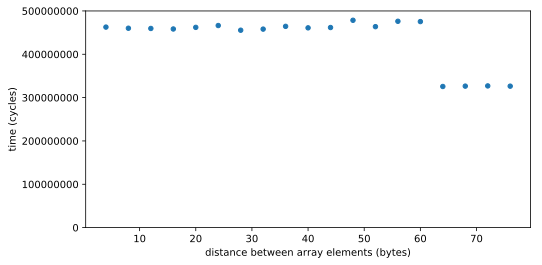
\includegraphics[width=\textwidth]{../sync/sum-up}
\end{frame}

\begin{frame}{false sharing}
\begin{itemize}
\item synchronizing to access two independent things
\vspace{.5cm}
\item two parts of same cache block
\item solution: separate them
\end{itemize}
\end{frame}

\subsubsection{exercise}
\begin{frame}[fragile,label=falseSharingEx1]{exercise (1)}
\begin{lstlisting}[
    language=C++,basicstyle=\tt\fontsize{9}{10}\selectfont,
    moredelim={**[is][\btHL<0|handout:0>]{@2}{2@}},
    moredelim={**[is][\btHL<0|handout:0>]{@3}{3@}},
    moredelim={**[is][\btHL<0|handout:0>]{@4}{4@}},
    escapeinside=QQ,
]
int @2values[1024]2@;
int @2results[2]2@;
void *sum_front(void *ignored_argument) {
    results[0] = 0;
    for (int i = @303@; i < @35123@; ++i)
        results[0] += values[i];
    return NULL;
}
void *sum_back(void *ignored_argument) {
    results[1] = 0;
    for (int i = @35123@; i < @310243@; ++i)
        results[1] += values[i];
    return NULL;
}
int sum_all() {
    pthread_t sum_front_thread, sum_back_thread;
    pthread_create(&sum_front_thread, NULL, sum_front, NULL);
    pthread_create(&sum_back_thread, NULL, sum_back, NULL);
    pthread_join(sum_front_thread, NULL);
    pthread_join(sum_back_thread, NULL);
    return @4results[0] + results[1]4@;
}
\end{lstlisting}
Where is false sharing likely to occur? How to fix?
\end{frame}

\begin{frame}[fragile,label=falseSharingEx2]{exercise (2)}
\begin{lstlisting}[
    language=C++,basicstyle=\tt\fontsize{9}{10}\selectfont,
    moredelim={**[is][\btHL<0|handout:0>]{@2}{2@}},
    moredelim={**[is][\btHL<0|handout:0>]{@3}{3@}},
    moredelim={**[is][\btHL<0|handout:0>]{@4}{4@}},
    escapeinside=QQ,
]
struct ThreadInfo { @2int *values;2@ int start; int end; int result };
void *sum_thread(void *argument) {
    ThreadInfo *@3my_info3@ = (ThreadInfo *) argument;Q\tikzmark{info}Q
    int sum = 0;
    for (int i = my_info->start; i < my_info->end; ++i) {
        my_info->result += my_info->values[i];
    }
    return NULL;

}
int sum_all(int *values) {
    ThreadInfo info[2]; pthread_t thread[2];
    for (int i = 0; i < 2; ++i) {
        @2info[i].values = values;2@ info[i].start = i*512; info[i].end = (i+1)*512;
        pthread_create(&threads[i], NULL, sum_thread, (void *) &info[i]);
    }
    for (int i = 0; i < 2; ++i)
        pthread_join(threads[i], NULL);
    return info[0].result + info[1].result;
}
\end{lstlisting}
Where is false sharing likely to occur?
\end{frame}



\subsection{exercise: ConsumeTwo}
\begin{frame}[fragile,label=monitorExercise]{monitor exercise: ConsumeTwo}
\begin{itemize}
\item suppose we want producer/consumer, but\ldots
\item but change Consume() to ConsumeTwo() which returns a \myemph{pair of values}
    \begin{itemize}
    \item and don't want two calls to ConsumeTwo() to wait\ldots
    \item with each getting one item
    \end{itemize}
\item what should we change below?
\end{itemize}
\begin{minipage}{0.45\textwidth}
\begin{lstlisting}[
    language=C++,
    basicstyle=\tt\fontsize{9.5}{10.5}\selectfont,
    morekeywords=pthread_mutex_t,
    morekeywords=pthread_cond_t,
    morekeywords=UnboundedQueue,
    moredelim={**[is][\btHL<2|handout:2>]{@2}{2@}}, 
    moredelim={**[is][\btHL<3|handout:3>]{@3}{3@}}, 
    moredelim={**[is][\btHL<4|handout:4>]{@4}{4@}}, 
    moredelim={**[is][\btHL<5-,3|handout:5-,3>]{@5}{5@}}, 
    escapeinside=XX,
]
pthread_mutex_t lock;
pthread_cond_t data_ready;
UnboundedQueue buffer;

Produce(item) {
  pthread_mutex_lock(&lock);
  buffer.enqueue(item);
  pthread_cond_signal(&data_ready);
  pthread_mutex_unlock(&lock);
}
\end{lstlisting}
\end{minipage}
\begin{minipage}{0.45\textwidth}
\begin{lstlisting}[
    language=C++,
    basicstyle=\tt\fontsize{9.5}{10.5}\selectfont,
    morekeywords=pthread_mutex_t,
    morekeywords=pthread_cond_t,
    morekeywords=UnboundedQueue,
    moredelim={**[is][\btHL<2|handout:2>]{@2}{2@}}, 
    moredelim={**[is][\btHL<3|handout:3>]{@3}{3@}}, 
    moredelim={**[is][\btHL<4|handout:4>]{@4}{4@}}, 
    moredelim={**[is][\btHL<5-,3|handout:5-,3>]{@5}{5@}}, 
    escapeinside=XX,
]
Consume() {
  pthread_mutex_lock(&lock);
  while (buffer.empty()) {
    pthread_cond_wait(&data_ready, &lock);
  }
  item = buffer.dequeue();
  pthread_mutex_unlock(&lock);
  return item;
}
\end{lstlisting}
\end{minipage}
\end{frame}

\iftoggle{heldback}{\excludecomment{isheldback}}{\includecomment{isheldback}}
\begin{isheldback}
\begin{frame}[fragile,label=monitorExerciseSln]{monitor exercise: solution (1)}
\small (one of many possible solutions) \\
Assuming ConsumeTwo \textbf{replaces} Consume:
\begin{lstlisting}[basicstyle=\tt\fontsize{9.5}{10.5}\selectfont]
Produce() {
  pthread_mutex_lock(&lock);
  buffer.enqueue(item);
  if (buffer.size() > 1) { pthread_cond_signal(&data_ready); }
  pthread_mutex_unlock(&lock);
}
ConsumeTwo() {
    pthread_mutex_lock(&lock);
    while (buffer.size() < 2) { pthread_cond_wait(&data_ready, &lock); }
    item1 = buffer.dequeue(); item2 = buffer.dequeue();
    pthread_mutex_unlock(&lock);
    return Combine(item1, item2);
}
\end{lstlisting}
\end{frame}

\begin{frame}[fragile,label=monitorExerciseSln2]{monitor exercise: solution (2)}
\small (one of many possible solutions) \\
Assuming ConsumeTwo is \textbf{in addition to} Consume (using two CVs):
\begin{lstlisting}[basicstyle=\tt\fontsize{9}{10}\selectfont]
Produce() {
  pthread_mutex_lock(&lock);
  buffer.enqueue(item);
  pthread_cond_signal(&one_ready);
  if (buffer.size() > 1) { pthread_cond_signal(&two_ready); }
  pthread_mutex_unlock(&lock);
}
Consume() {
  pthread_mutex_lock(&lock);
  while (buffer.size() < 1) { pthread_cond_wait(&one_ready, &lock); }
  item = buffer.dequeue();
  pthread_mutex_unlock(&lock);
  return item;
}
ConsumeTwo() {
  pthread_mutex_lock(&lock);
  while (buffer.size() < 2) { pthread_cond_wait(&two_ready, &lock); }
  item1 = buffer.dequeue(); item2 = buffer.dequeue();
  pthread_mutex_unlock(&lock);
  return Combine(item1, item2);
}
\end{lstlisting}
\end{frame}

\begin{frame}[fragile,label=monitorExerciseSln3]{monitor exercise: slower solution}
\small (one of many possible solutions) \\
Assuming ConsumeTwo is \textbf{in addition to} Consume (using one CV):
\begin{lstlisting}[basicstyle=\tt\fontsize{9}{10}\selectfont]
Produce() {
  pthread_mutex_lock(&lock);
  buffer.enqueue(item);
  // broadcast and not signal, b/c we might wakeup only ConsumeTwo() otherwise
  pthread_cond_broadcast(&data_ready);
  pthread_mutex_unlock(&lock);
}
Consume() {
  pthread_mutex_lock(&lock);
  while (buffer.size() < 1) { pthread_cond_wait(&data_ready, &lock); }
  item = buffer.dequeue();
  pthread_mutex_unlock(&lock);
  return item;
}
ConsumeTwo() {
  pthread_mutex_lock(&lock);
  while (buffer.size() < 2) { pthread_cond_wait(&data_ready, &lock); }
  item1 = buffer.dequeue(); item2 = buffer.dequeue();
  pthread_mutex_unlock(&lock);
  return Combine(item1, item2);
}
\end{lstlisting}
\end{frame}
\end{isheldback}



\subsection{exercise: conditional signal in produce?}
\begin{frame}[fragile,label=PCSignal]{producer/consumer signal?}
\begin{lstlisting}[
    language=C++,
    basicstyle=\tt\fontsize{9.5}{10.5}\selectfont,
    morekeywords=pthread_mutex_t,
    morekeywords=pthread_cond_t,
    morekeywords=BoundedQueue,
    moredelim={**[is][\btHL<0|handout:0>]{@2}{2@}}, 
    moredelim={**[is][\btHL<0|handout:0>]{@3}{3@}}, 
    moredelim={**[is][\btHL<0|handout:0>]{@4}{4@}}, 
    moredelim={**[is][\btHL<0|handout:0>]{@5}{5@}}, 
    escapeinside=XX,
]
pthread_mutex_t lock;
pthread_cond_t data_ready;
UnboundedQueue buffer;

Produce(item) {
    @2pthread_mutex_lock(&lock);2@
    buffer.enqueue(item);
    /* GOOD CODE: pthread_cond_signal(&data_ready); */
    /* BAD CODE: */
    if (buffer.size() == 1)
        pthread_cond_signal(&item);
    @2pthread_mutex_unlock(&lock);2@
}

Consume() {
    @2pthread_mutex_lock(&lock);2@
    while (@5buffer.empty()5@) {X\tikzmark{empty}X
        pthread_cond_wait(&data_ready, &lock);
    }X\tikzmark{after loop}X
    item = @3buffer.dequeue()3@;
    @2pthread_mutex_unlock(&lock);2@
    return item;
}
\end{lstlisting}
\begin{itemize}
    \item exercise: come up with scenario in which this doesn't work.
        \begin{itemize}
        \item hint 1: assume two waiting consume()s, and two produce() calls
        \item hint 2: related to Mesa-style versus Hoare-style 
            \begin{itemize}
            \item signaling thread $\not\implies$ thread gets lock next
            \end{itemize}
        \end{itemize}
\end{itemize}
\end{frame}

\begin{frame}<0>[fragile,label=PCSignalBadSetup]{bad case (setup)}
\fontsize{12}{13}\selectfont
\begin{tabular}{l|l|l|l}
thread 0 & 1 & 2 & 3 \\ \hline
Consume(): & & \\
lock & & \\
empty? wait on cv & Consume(): \\
     & lock & \\
     & empty? wait on cv & & \\
     & & Produce(): & \\
     & & lock & Produce(): \\
\end{tabular}
\end{frame}

\againframe<1>{PCSignalBadSetup}

\begin{frame}<0>[fragile,label=PCSignalBad]{bad case}
\fontsize{12}{13}\selectfont
\begin{tabular}{l|l|l|l}
thread 0 & 1 & 2 & 3 \\ \hline
Consume(): & & \\
lock & & \\
empty? wait on cv & Consume(): \\
     & lock & \\
     & empty? wait on cv & & \\
     & & Produce(): & \\
     & & lock & Produce(): \\
     & & & wait for lock \\
     & & enqueue & \\
wait for lock & & size = 1? signal \\
              & & unlock & gets lock \\
              & & & enqueue \\
              & & & \myemph{size $\not=$ 1}: don't signal \\
              & & & unlock \\
gets lock & & & \\
dequeue & & &\\
& still waiting & &
\end{tabular}
\end{frame}

\againframe<1>{PCSignalBad}


\subsection{exercise: ConsumeTwo}
\begin{frame}[fragile,label=monitorExercise]{monitor exercise: ConsumeTwo}
\begin{itemize}
\item suppose we want producer/consumer, but\ldots
\item but change Consume() to ConsumeTwo() which returns a \myemph{pair of values}
    \begin{itemize}
    \item and don't want two calls to ConsumeTwo() to wait\ldots
    \item with each getting one item
    \end{itemize}
\item what should we change below?
\end{itemize}
\begin{minipage}{0.45\textwidth}
\begin{lstlisting}[
    language=C++,
    basicstyle=\tt\fontsize{9.5}{10.5}\selectfont,
    morekeywords=pthread_mutex_t,
    morekeywords=pthread_cond_t,
    morekeywords=UnboundedQueue,
    moredelim={**[is][\btHL<2|handout:2>]{@2}{2@}}, 
    moredelim={**[is][\btHL<3|handout:3>]{@3}{3@}}, 
    moredelim={**[is][\btHL<4|handout:4>]{@4}{4@}}, 
    moredelim={**[is][\btHL<5-,3|handout:5-,3>]{@5}{5@}}, 
    escapeinside=XX,
]
pthread_mutex_t lock;
pthread_cond_t data_ready;
UnboundedQueue buffer;

Produce(item) {
  pthread_mutex_lock(&lock);
  buffer.enqueue(item);
  pthread_cond_signal(&data_ready);
  pthread_mutex_unlock(&lock);
}
\end{lstlisting}
\end{minipage}
\begin{minipage}{0.45\textwidth}
\begin{lstlisting}[
    language=C++,
    basicstyle=\tt\fontsize{9.5}{10.5}\selectfont,
    morekeywords=pthread_mutex_t,
    morekeywords=pthread_cond_t,
    morekeywords=UnboundedQueue,
    moredelim={**[is][\btHL<2|handout:2>]{@2}{2@}}, 
    moredelim={**[is][\btHL<3|handout:3>]{@3}{3@}}, 
    moredelim={**[is][\btHL<4|handout:4>]{@4}{4@}}, 
    moredelim={**[is][\btHL<5-,3|handout:5-,3>]{@5}{5@}}, 
    escapeinside=XX,
]
Consume() {
  pthread_mutex_lock(&lock);
  while (buffer.empty()) {
    pthread_cond_wait(&data_ready, &lock);
  }
  item = buffer.dequeue();
  pthread_mutex_unlock(&lock);
  return item;
}
\end{lstlisting}
\end{minipage}
\end{frame}

\iftoggle{heldback}{\excludecomment{isheldback}}{\includecomment{isheldback}}
\begin{isheldback}
\begin{frame}[fragile,label=monitorExerciseSln]{monitor exercise: solution (1)}
\small (one of many possible solutions) \\
Assuming ConsumeTwo \textbf{replaces} Consume:
\begin{lstlisting}[basicstyle=\tt\fontsize{9.5}{10.5}\selectfont]
Produce() {
  pthread_mutex_lock(&lock);
  buffer.enqueue(item);
  if (buffer.size() > 1) { pthread_cond_signal(&data_ready); }
  pthread_mutex_unlock(&lock);
}
ConsumeTwo() {
    pthread_mutex_lock(&lock);
    while (buffer.size() < 2) { pthread_cond_wait(&data_ready, &lock); }
    item1 = buffer.dequeue(); item2 = buffer.dequeue();
    pthread_mutex_unlock(&lock);
    return Combine(item1, item2);
}
\end{lstlisting}
\end{frame}

\begin{frame}[fragile,label=monitorExerciseSln2]{monitor exercise: solution (2)}
\small (one of many possible solutions) \\
Assuming ConsumeTwo is \textbf{in addition to} Consume (using two CVs):
\begin{lstlisting}[basicstyle=\tt\fontsize{9}{10}\selectfont]
Produce() {
  pthread_mutex_lock(&lock);
  buffer.enqueue(item);
  pthread_cond_signal(&one_ready);
  if (buffer.size() > 1) { pthread_cond_signal(&two_ready); }
  pthread_mutex_unlock(&lock);
}
Consume() {
  pthread_mutex_lock(&lock);
  while (buffer.size() < 1) { pthread_cond_wait(&one_ready, &lock); }
  item = buffer.dequeue();
  pthread_mutex_unlock(&lock);
  return item;
}
ConsumeTwo() {
  pthread_mutex_lock(&lock);
  while (buffer.size() < 2) { pthread_cond_wait(&two_ready, &lock); }
  item1 = buffer.dequeue(); item2 = buffer.dequeue();
  pthread_mutex_unlock(&lock);
  return Combine(item1, item2);
}
\end{lstlisting}
\end{frame}

\begin{frame}[fragile,label=monitorExerciseSln3]{monitor exercise: slower solution}
\small (one of many possible solutions) \\
Assuming ConsumeTwo is \textbf{in addition to} Consume (using one CV):
\begin{lstlisting}[basicstyle=\tt\fontsize{9}{10}\selectfont]
Produce() {
  pthread_mutex_lock(&lock);
  buffer.enqueue(item);
  // broadcast and not signal, b/c we might wakeup only ConsumeTwo() otherwise
  pthread_cond_broadcast(&data_ready);
  pthread_mutex_unlock(&lock);
}
Consume() {
  pthread_mutex_lock(&lock);
  while (buffer.size() < 1) { pthread_cond_wait(&data_ready, &lock); }
  item = buffer.dequeue();
  pthread_mutex_unlock(&lock);
  return item;
}
ConsumeTwo() {
  pthread_mutex_lock(&lock);
  while (buffer.size() < 2) { pthread_cond_wait(&data_ready, &lock); }
  item1 = buffer.dequeue(); item2 = buffer.dequeue();
  pthread_mutex_unlock(&lock);
  return Combine(item1, item2);
}
\end{lstlisting}
\end{frame}
\end{isheldback}


\subsection{exercise: ordering}
\begin{frame}[fragile,label=monitorOrderExercise]{monitor exercise: ordering}
\begin{itemize}
\item suppose we want producer/consumer, but\ldots
\item but want to ensure first call to Consume() \textbf{always} returns first
\item (no matter what ordering cond\_signal/cond\_broadcast use)
\end{itemize}
\begin{tikzpicture}
\node (produce) {
\begin{lstlisting}[
    language=C++,
    basicstyle=\tt\fontsize{9.5}{10.5}\selectfont,
    morekeywords=pthread_mutex_t,
    morekeywords=pthread_cond_t,
    morekeywords=UnboundedQueue,
    moredelim={**[is][\btHL<2|handout:2>]{@2}{2@}}, 
    moredelim={**[is][\btHL<3|handout:3>]{@3}{3@}}, 
    moredelim={**[is][\btHL<4|handout:4>]{@4}{4@}}, 
    moredelim={**[is][\btHL<5-,3|handout:5-,3>]{@5}{5@}}, 
    escapeinside=XX,
]
pthread_mutex_t lock;
pthread_cond_t data_ready;
UnboundedQueue buffer;

Produce(item) {
  pthread_mutex_lock(&lock);
  buffer.enqueue(item);
  pthread_cond_signal(&data_ready);
  pthread_mutex_unlock(&lock);
}
\end{lstlisting}
};
\node[anchor=north west] at (produce.north east) {
\begin{lstlisting}[
    language=C++,
    basicstyle=\tt\fontsize{9.5}{10.5}\selectfont,
    morekeywords=pthread_mutex_t,
    morekeywords=pthread_cond_t,
    morekeywords=UnboundedQueue,
    moredelim={**[is][\btHL<2|handout:2>]{@2}{2@}}, 
    moredelim={**[is][\btHL<3|handout:3>]{@3}{3@}}, 
    moredelim={**[is][\btHL<4|handout:4>]{@4}{4@}}, 
    moredelim={**[is][\btHL<5-,3|handout:5-,3>]{@5}{5@}}, 
    escapeinside=XX,
]
Consume() {
  pthread_mutex_lock(&lock);
  while (buffer.empty()) {
    pthread_cond_wait(&data_ready, &lock);
  }
  item = buffer.dequeue();
  pthread_mutex_unlock(&lock);
  return item;
}
\end{lstlisting}
};
\end{tikzpicture}
\end{frame}

\iftoggle{heldback}{\excludecomment{isheldback}}{\includecomment{isheldback}}
\begin{isheldback}
\begin{frame}[fragile,label=monitorOrderExerciseSln]{monitor ordering exercise: solution}
\small (one of many possible solutions) \\
\begin{tikzpicture}
\node (produce) {
\begin{lstlisting}[basicstyle=\tt\fontsize{9.5}{10.5}\selectfont]
struct Waiter {
    pthread_cond_t cv;
    bool done;
    T item;    
}
Queue<Waiter*> waiters;

Produce(item) {
 pthread_mutex_lock(&lock);
 if (!waiters.empty()) {
   Waiter *waiter = waiters.dequeue();
   waiter->done = true;
   waiter->item = item;
   cond_signal(&waiter->cv);
   ++num_pending;
 } else {
   buffer.enqueue(item);
 }
 pthread_mutex_unlock(&lock);
}
\end{lstlisting}
};
\node[anchor=north west] (consume) at (produce.north east) {
\begin{lstlisting}[basicstyle=\tt\fontsize{9.5}{10.5}\selectfont]
Consume() {
  pthread_mutex_lock(&lock);
  if (buffer.empty()) {
    Waiter waiter;
    cond_init(&waiter.cv);
    waiter.done = false;
    waiters.enqueue(&waiter);
    while (!waiter.done)
      cond_wait(&waiter.cv, &lock);
    item = waiter.item;
  } else {
    item = buffer.dequeue();
  }
  pthread_mutex_unlock(&lock):
  return item;
}
\end{lstlisting}
};
\end{tikzpicture}
\end{frame}
\end{isheldback}




\subsection{link layer quality-of-service}

\begin{frame}{link layer quality of service}
if frame gets\ldots \\
\small
\begin{tabular}{l|l|l}
event & on Ethernet & on WiFi \\\hline
collides with another & detected + may resend & resend\\
not received & lose silently & resent \\
header corrupted & usually discard silently & usually resend \\
data corrupted & usually discard silently & usually resend \\
too long & not allowed to send & not allowed to send \\
reordered (v. other messages)  & received out of order & received out of order \\
destination unknown & lose silently & usually resend?? \\
too much being sent & discard excess? & discard excess? \\
\end{tabular}
\end{frame}


\subsection{network layer quality-of-service}

\begin{frame}[fragile]{network layer quality of service}
if packet \ldots \\
\small
\begin{tabular}{l|p{12cm}}
event & on IPv4/v6 \\\hline
collides with another & out of scope --- handled by link layer \\
\myemph<2>{not received}\tikzmark{not recv} & lost silently \\
header corrupted & usually discarded silently \\
data corrupted & received corrupted \\
too long & dropped with notice or ``fragmented'' + recombined \\
reordered (v. other messages) & received out of order \\
destination unknown & usually dropped with notice \\
too much being sent & discard excess \\
\end{tabular}
\begin{tikzpicture}[overlay,remember picture]
\begin{visibleenv}<2>
\node[align=left,my callout=not recv,anchor=north west] at ([xshift=0cm,yshift=-3cm]pic cs:not recv) {
    includes dropped by link layer \\
    (e.g. if detected corrupted there)
};
\end{visibleenv}
\end{tikzpicture}
\end{frame}


\subsection{UDP sockets}

\begin{frame}[fragile]{`connected' UDP sockets}
\begin{lstlisting}[language=C++,style=smaller]
int fd = socket(AF_INET, SOCK_DGRAM, 0);
struct sockaddr_in my_addr= ...;
bind(fd, &my_addr, sizeof(my_addr))
struct sockaddr_in to_addr = ...;
connect(fd, &to_addr);
...
int count = write(fd, data, data_size);
// OR
int count = send(fd, data, data_size, 0 /* flags */);

int count = read(fd, buffer, buffer_size);
// OR
int count = recv(fd, buffer, buffer_size, 0 /* flags */);
\end{lstlisting}
\end{frame}

\begin{frame}[fragile]{UDP sockets on IPv4}
\begin{lstlisting}[language=C++,style=smaller]
int fd = socket(AF_INET, SOCK_DGRAM, 0);
struct sockaddr_in my_addr= ...;
if (0 != bind(fd, &my_addr, sizeof(my_addr)))
    handle_error();
...
struct sockaddr_in to_addr = ...;
int bytes_sent = sendto(fd, data, data_size, 0 /* flags */,
    &to_addr, sizeof(to_addr));
struct sockaddr_in from_addr = ...;
iint bytes_recvd = recvfrom(fd, &buffer[0], buffer_size, 0,
    &from_addr, sizeof(from_addr));
...
\end{lstlisting}
\end{frame}


\subsection{example: echo client/server}
\subsubsection{server setup}
\input{../network/conn-setup-server-manual}
\subsubsection{client setup}
\input{../network/conn-setup-client-manual}

\subsubsection{read/write code}

\begin{frame}[fragile,label=echoClient]{echo client/server}
\begin{lstlisting}[
    language=C++,
    basicstyle=\sourcecodepro\EmptyMapping\fontsize{10}{11}\selectfont,
    keywordstyle=\sourcecodepro\EmptyMapping\fontsize{10}{11}\selectfont,
    moredelim={**[is][\btHL<1|handout:1>]{@1}{1@}},
    moredelim={**[is][\btHL<2|handout:2>]{@2}{2@}},
    moredelim={**[is][\btHL<3|handout:3>]{@3}{3@}},
    moredelim={**[is][\btHL<4|handout:4>]{@4}{4@}},
    moredelim={**[is][\btHL<5|handout:5>]{@5}{5@}},
    moredelim={**[is][\btHL<6|handout:6>]{@6}{6@}},
]
void client_for_connection(int socket_fd) {
    int n; char send_buf[MAX_SIZE]; char recv_buf[MAX_SIZE];
    while (prompt_for_input(send_buf, MAX_SIZE)) {
        n = @2write(socket_fd, send_buf, strlen(send_buf))2@;
        if (n != strlen(send_buf)) {...error?...}
        n = @3read(socket_fd, recv_buf, MAX_SIZE)3@;
        if (n <= 0) return; // error or EOF 
        write(STDOUT_FILENO, recv_buf, n);
    }
}
\end{lstlisting}
\hrule
\begin{lstlisting}[
    language=C++,style=smaller,
    moredelim={**[is][\btHL<1|handout:1>]{@1}{1@}},
    moredelim={**[is][\btHL<2|handout:2>]{@2}{2@}},
    moredelim={**[is][\btHL<3|handout:3>]{@3}{3@}},
    moredelim={**[is][\btHL<4|handout:4>]{@4}{4@}},
    moredelim={**[is][\btHL<5|handout:5>]{@5}{5@}},
    moredelim={**[is][\btHL<6|handout:6>]{@6}{6@}},
]
void server_for_connection(int socket_fd) {
    int read_count, write_count; char request_buf[MAX_SIZE];
    while (1) {
        read_count = @2read(socket_fd, request_buf, MAX_SIZE)2@;
        if (read_count <= 0) return; // error or EOF 
        write_count = @3write(socket_fd, request_buf, read_count)3@;
        if (read_count != write_count) {...error?...}
    }
}
\end{lstlisting}
\end{frame}



\subsection{more normal connection setup}
\input{../network/conn-setup-server}
\input{../network/conn-setup-client}

\subsection{other connection setup options}
\input{../network/conn-setup-server-multi}
\input{../network/conn-setup-gethostbyname}
\input{../network/conn-setup-server-1023-note}



\begin{frame}{implementing consistency: simple}
    \begin{itemize}
    \item simplest idea: only one run transaction at a time
    \end{itemize}
\end{frame}

\begin{frame}{implementing consistency: locking}
    \begin{itemize}
    \item everytime something read/written: acquire associated lock
    \item on end transaction: release lock
    \vspace{.5cm}
    \item if deadlock: \myemph<2>{undo everything}, go back to BeginTransaction(), retry
        \begin{itemize}
        \item how to undo?
        \item one idea: keep list of writes instead of writing
        \item apply writes only at EndTransaction()
        \end{itemize}
    \end{itemize}
\end{frame}

\begin{frame}{implementing consistency: optimistic}
    \begin{itemize}
    \item on read: copy version \# for value read 
    \item on write: record value to be written, but don't write yet
    \item on end transaction: 
        \begin{itemize}
        \item acquire locks on everything
        \item make sure values read haven't been changed since read
        \end{itemize}
    \vspace{.5cm}
    \item if they have changed, just retry transaction
    \end{itemize}
\end{frame}



\end{document}
